\section{Funktionsweise der Werkzeuge}

Dieses Kapitel erläutet die interne Funktionsweise der gebräuchlichsten statischen Code Analyse Tools für Java. Diese sind wie in vorherigen Kapiteln dargestellt: Findbugs, Checkstyle, PMD sowie Emma, welches den Code zwar nicht statisch analysiert, im Rahmen der Vorlesung aber trotzdem im Kontext der statischen Analyse besprochen wurde.


\subsection{FindBugs}

FindBugs ist ein von der Universität von Maryland initiiertes Software-Projekt zur statischen Code Analyse. FindBugs ist in der Industrie weit verbreitet im Einsatz und wird von Firmen wie Google und Oracle (ehemals Sun Microsystems) unterstüzt.
FindBugs arbeitet vollständig auf dem Java-Bytecode und kann dadurch auch ``binäre'' Projektdistributionen analysieren. 

FindBugs bietet eine große Anzahl an mitgelieferten Fehlermustern, die in verschiedene Warnstufen eingeteilt sind. Ihr Hauptfokus liegt auf der Erkennung von fehlerhaftem Code, der bei der Ausführung zu Laufzeitfehlern führen würde.

Möchte man seine eigenen Fehlermuster (Patterns) hinzufügen, so bietet Findbugs dafür ein Plugin-Konzept, welches allerdings ein Verständnis der internen Funktionsweise von FindBugs voraussetzt.
 
FindBugs nutzt für die Bytecode-Analyse die \textit{Apache BCEL Library}\footnote{Byte Code Engineering Library}. Diese bietet eine gut nutzbare Schnittstelle zu kompilierten Java-Class-Dateien, welche in vielen Bytecode-nahen Projekten eingesetzt wird. % "zu" class-Dateien oder "für"?

Dies kann für Entwickler einen großen Nachteil bedeuten, da die Wenigsten ein Verständnis von Bytecode haben. Man muss beachten, dass die baumartige Struktur des Quellcodes im Bytecode -- wie auch in Maschinensprache -- zu einer flachen sequenziellen Abfolge von Instruktionen wird. 

Zudem erschwert das Erstellen eines eigenen Fehlermusters dass der Bytecode sequenziell Durchlaufen wird und der Bytecode-Scanner dabei bei jeder Instruktion die ihm zugeordnenten Fehler-Detektoren über ein Visitor-Pattern aufruft. 
Dadurch ist der Entwickler des Fehler-Detektors dafür verantwortlich, sich die bereits gescannten Instruktionen in seinem Zustand zu speichern. Hierfür bietet sich in der Regel eine Zustandsmaschine an. Auch dies ist jedoch ein Programmierparadigma, das bei vielen Entwicklern in Zeiten von objektorientierter Programmierung nicht mehr häufig genutzt wird und somit eine weitere Hürde in der Erstellung von eigenen Fehler-Mustern darstellt.

Die Analyse des Bytecodes hat aber auch positive Seiten. So ist zum Einen die Analyse sehr performant, da sie einfach einer linearen Abarbeitung von Instruktionen entspricht. Zum Anderen ist der Bytecode bereits durch den Java Compiler optimiert worden und somit verringert sich die Häufigkeit eines \textit{False-Positive}.

Hinsichtlich seiner Benutzerfreundlichkeit bietet FindBugs auch Vorteile gegenüber anderen Werkzeugen. So bietet es zum Einen eine sehr gute und aktuelle Integration in Eclipse und viele andere Entwicklungsumgebungen und lässt sich zum Anderen über ein Konsolen-Tool einfach in automatische Build-Prozesse einbinden.


\subsection{PMD}
PMD, dessen Name nach eigenen Aussagen des Projektteams keine ausgeschriebe Bedeutung hat, ist ebenfalls ein Werkzeug zur statischen Code Analyse von Java-Quellcode. 

Auch PMD liefert eine Vielzahl an eingebauten Regeln, die anders als bei FindBugs nicht so sehr auf potentielle Fehler, sondern eher auf ineffizienten Code ausgelegt sind. Beispiele hierfür sind z.B. leere Blöcke, toter Code oder die falsche Verwendung von \verb=String= und \verb=StringBuffer=. 

PMD besitzt weiter einen Copy/Paste-Detektor, der es erlaubt, mithilfe des Rabin-Karp-Algorithmus' duplizierten Code zu finden.

PMD arbeitet, anders als FindBugs, nicht auf den binären Java Class-Dateien, sondern auf dem Quellcode. Genauer gesagt analysiert PMD auf der Ebene des \textit{Abstract Syntax Tree} (AST), der aus dem Quellcode vor dem Erstellen des Bytecode erzeugt wird. 

Die Analyse des ASTs ist zwar nicht so performant wie das einfache Scannen von Bytecode, besitzt für das Entwicklen von eigenen Regeln aufgrund der Nähe zum Quellcode aber entsprechende Vorteile.

Bei der Transformation des Quelltextes zu einem Abstract Syntax Tree gehen im Gegensatz zu Bytecode keine Informationen über die Struktur des Quelltextes verloren. Es wird einzig der vorhandene Quelltext in einem Baum abgebildet. 
Möchte man nun seine eigenen PMD Regeln hinzufügen, reicht es aus den AST zu traversieren und auf das Vorkommen des entsprechenden Musters zu untersuchen. PMD bietet für diese Aufgabe ein eigenes Entwicklungstool an, das den erzeugten AST darstellt, und in dem man explorativ diese Baumstruktur traversieren kann.

\begin{figure}[htbp]
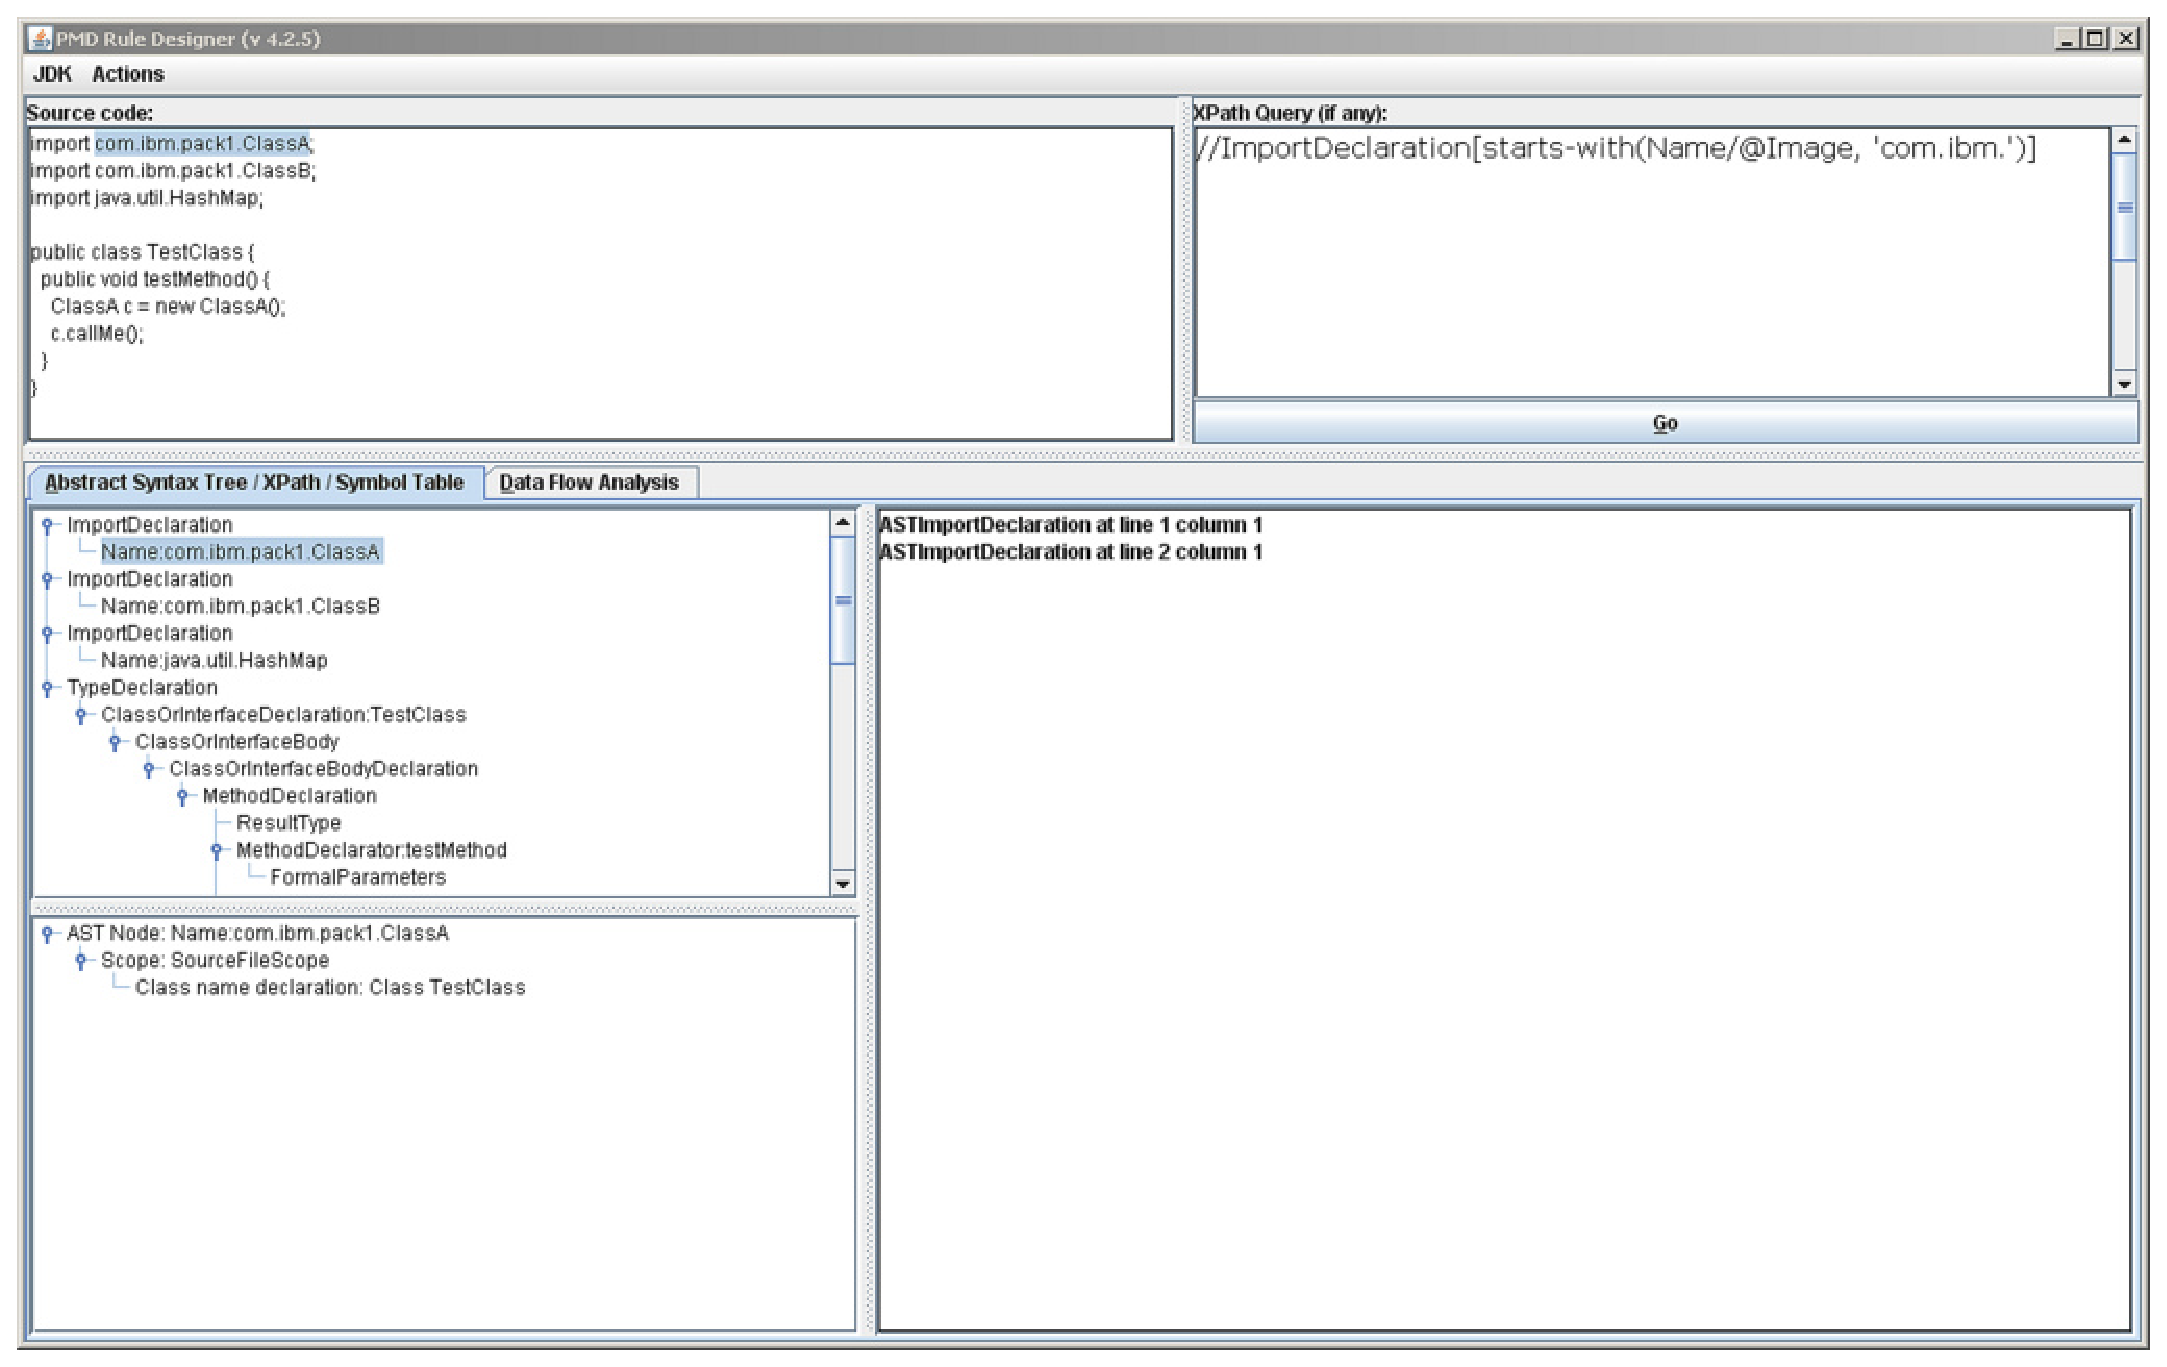
\includegraphics[width=10cm]{pmd-dev}
\caption{Bildschirmfoto des Entwicklungswerkzeugs PMD}
\end{figure}

Die Analyse auf einem AST bietet einen weiteren Vorteil: Da Bäume eine weit verbreitete Darstellungsform sind, gibt es bereits eine Vielzahl von Werkzeugen die auf ihnen operieren können. Das in diesem Kontext wichtigste Werkzeug ist \textit{XPath}.

PMD bietet neben der Schnitstelle für in Java implementierte Regeln auch eine Schnittstelle für XPath an.

XPath oder auch \textit{XML Path Language} ist eine vom W3-Konsortium entwickelte Abfragesprache, um Teile eines XML-Dokumentes abzufragen, welche ebenfalls Bäume sind. Dabei bietet es eine sehr einfache Möglichkeit, Bäume zu travasieren. Das folgende Beispiel würde z.B. alle Bücher aus einem Baum liefern, das maximal 100, jedoch mindestens 10 Kindelemente/Seiten hat:


\begin{lstlisting}
//child:Buch[count(./Seite)<=100]
/count(.Seite)>=10]
\end{lstlisting}

Diese XPath-Ausdrücke können direkt in den PMD-Konfigurations-Dateien angegeben werden und machen es so für einfache und mittelmäßig komplexe Regeln überflüssig, eigene Java-Module zu implementieren.

PMD bietet ebenfalls ein Konsolen-Tool, das sich sehr gut in Build-Prozesse integrieren lässt. Das entsprechende Eclipse Plugin ist zum aktuellen Zeitpunkt (Juli 2012) leider nicht auf dem aktuellsten Stand: Es arbeitet noch mit PMD Version 4, welche zur Version 5 inkompatibele Konfigurations-Dateien nutzt. Soll also die aktuellste PMD Version 5 im Build-Prozess verwendet werden, müssen zwei Konfigurations-Dateien für Version 4 und 5 gepflegt werden.


\subsection{Checkstyle}

Checkstyle ist das dritte wichtige Werkzeug zur statischen Code Analyse in der Java-Welt. Der Fokus von Checkstyle liegt weder in der effizenten Nutzung der JVM noch in dem Auffinden von Programmierfehlern, sondern vor allem in der Prüfung des Quellcodes auf die Einhaltung eines einheitlichen Programmierstils. 
Dafür liefert Checkstyle viele Regeln von Haus aus mit, die in Modulen gruppiert sind. Einige Beispiele an mitgliefierten Modulen sind:
\begin{itemize}
\item \textit{Class Design}, welches Prüfungen zum Softwaredesign beinhaltet
\item \textit{Coding}, das allgemeine Coding Guidelines prüft
\item \textit{Javadoc Comments} zum Prüfen der Vollständigkeit und der richtigen Formatierung von Javadoc-Kommentaren
\item \textit{Metrics} zum Sicherstellen der  Einhaltung diverser Sofwaremetriken
\item \textit{Naming Conventions}, um die Einhaltung von Namenskonventionen zu prüfen
\item \textit{Whitspaces} zur Prüfung des Quelltextes hinsichtlich Leerzeichen und korrekter Einrückung
\end{itemize}
Checksyle arbeitet ähnlich wie PMD auf dem AST und kann durch eigene Java-Module erweitert werden, die ebenfalls auf dem AST arbeiten. Checkstyle bietet zur Erweierung noch eine weitere sehr nützliche Schnitstelle. So bietet das Modul ``Regexp'' es dem Entwickler an, eigene Regeln mithilfe von regulären Ausdrücken zu schreiben. Dies dürfte gerade beim Überprüfen von Coding Guildelines oft als ausreichend empfunden werden und bietet eine sehr einfache Schnittstelle, um Checkstyle zu erweitern.

Checkstyle lässt sich wie PMD und FindBugs sehr einfach über ein Konsolen-Werkzeug in den Build-Prozess einbinden und bietet ein gut funktionierendes Eclipse-Plugin.


\subsection{Emma}

Emma ist eine Code Coverage Library von Vlad Roubtsov. Sie zählt eigentlich nicht zu den statischen Code Analyse Tools, soll aber, da sie im Rahmen der Vorlesung im Kontext solcher behandelt wurde, hier kurz erläutert und zur statischen Code Analyse abgegrenzt werden. 
Das Ziel von Emma ist zu analysieren, welcher Code durchlaufen wird. Diese Information ist zum Beispiel für die Ermittlung einer Testabdeckung sehr interessant. Emma untersützt dabei eine Vielzahl von Metriken, die aber in den entsprechenden Ausarbeitungen zum Thema Testabdeckung zu finden sind. In diesem Kontext soll nun auf die Funktionsweise von Emma eingegangen werden.

Wie bereits erwähnt, ist Emma kein Werkzeug der statischen Code-Analyse. Die Funktionsweise von Emma basiert auf der Instrumentierung von Java Bytecode. Dazu untersützt Emma zwei Verfahren. Zum einen kann in einem zweiten "compile" Schritt der Bytecode um entsprechende Hooks erweitert werden, die dem Emma Toolkit die nötigen Daten über den durchlaufenden Code geben, und zum Anderen kann die Applikation mit einem speziellen Emma-Classloader gestartet werden, der den geladenen Bytecode on-the-fly instrumentiert. Als nächstes wird ein Driver benötigt, der den Instrumentierten Code durchläuft. Dies kann sowohl durc ein manuelles bedienen der Applikation geschehen, als auch durch automatische Tests. Der am weitestverbreiteste Anwendungsfall ist wohl die bereits erwähnte Testabdeckung bei Unit-Tests. Aber als reines Code Coverage Tool ist Emma natürlich wesentlich vielseitiger. So kann ein weiterer Interessanter Ansatz sein, dass man sich in (geerbtem) Spagetthi-Code einen schnellen Überblick verschaffen will, welcher Code bei einer Benutzeraktion durchlaufen wird.

Emma lässt sich über Ant und Maven Plugins gut in den BuildProzess inegrieren und bietet gerade für den Fall der Testabdeckung mit EclEmma ein sehr gutes Eclipse Plugin.

